\chapter{Constructing Structural Generalizations} \label{ch4} \label{methodology}

In Chapter~\ref{background}, I provided background information on higher-order anti-unification modulo theories, a theoretical framework that can be used to construct a generalization from two given ASTs. I also presented the framework proposed by \citet{2008:fse:cottrell} to construct the CAST structure, where each node holds a list of candidate structural correspondences in Chapter~\ref{background2}. I next extended the CAST structure to AUAST that would allow the creation of an anti-unifier. I now consider how these frameworks could help me (1)~to construct an approximation of the best anti-unifier to my problem from the AUASTs of two logged methods with special attention to log statements and (2)~to develop a similarity measure between the two structures, which can provide us with useful information for clustering a set of logged methods in a later phase. The constructed anti-unifier can be viewed as a generalization that represents the structural commonalities and differences between the two logged methods.


%I also described how Jigsaw applies this framework on ASTs of a pair of \name{Java} methods to determine candidate structural correspondences.

%To this end, first we should create an extended form of AST, called AUAST (Anti-unifier AST) that allows the insertion of variables in place of any node in the tree, which is a requirement for HOAUMT (see Section~\ref{AUAST}).
%1) generates all possible candidate correspondence connections between the two AUASTs using the Jigsaw framework (line~1) (see Section~\ref{meth-CAST});

To approximate the best anti-unifier for my problem, I should develop a greedy selection algorithm that determines the best correspondence for each node. My approach contains a sequence of 2 actions to find the best correspondences between two AUASTs: (1) it applies two constraints to prevent the anti-unification of log statement nodes with any other nodes; and (2) it determines the best correspondence for each AUAST node with the highest similarity and then removes the other correspondence connections involving those nodes (Section~\ref{best-corr}). However, to construct an anti-unifier, a further step should be taken, which is the anti-unification of each AUAST node with its best correspondence (Section~\ref{meth-antiUnifier}). Furthermore, I developed an algorithm to measure similarity between the usage of logging calls in methods based on the selected correspondences (Section~\ref{meth-similarity}). An overview of the proposed anti-unification approach is shown in Figure~\ref{fig:meth_overview}.





%computed the ratio of the number of common elements over the total number of elements of the anti-unifier to measure similarity between two AUASTs (see Section~\ref{meth-similarity}).
%I computed the ratio of the number of common elements over the total number of elements of the anti-unifier to measure similarity between two AUASTs (see Section~\ref{meth-similarity}).
%(Section ~\ref{meth-constraints})
%through anti-unifying their structural properties



\begin{figure} [H]
  \centering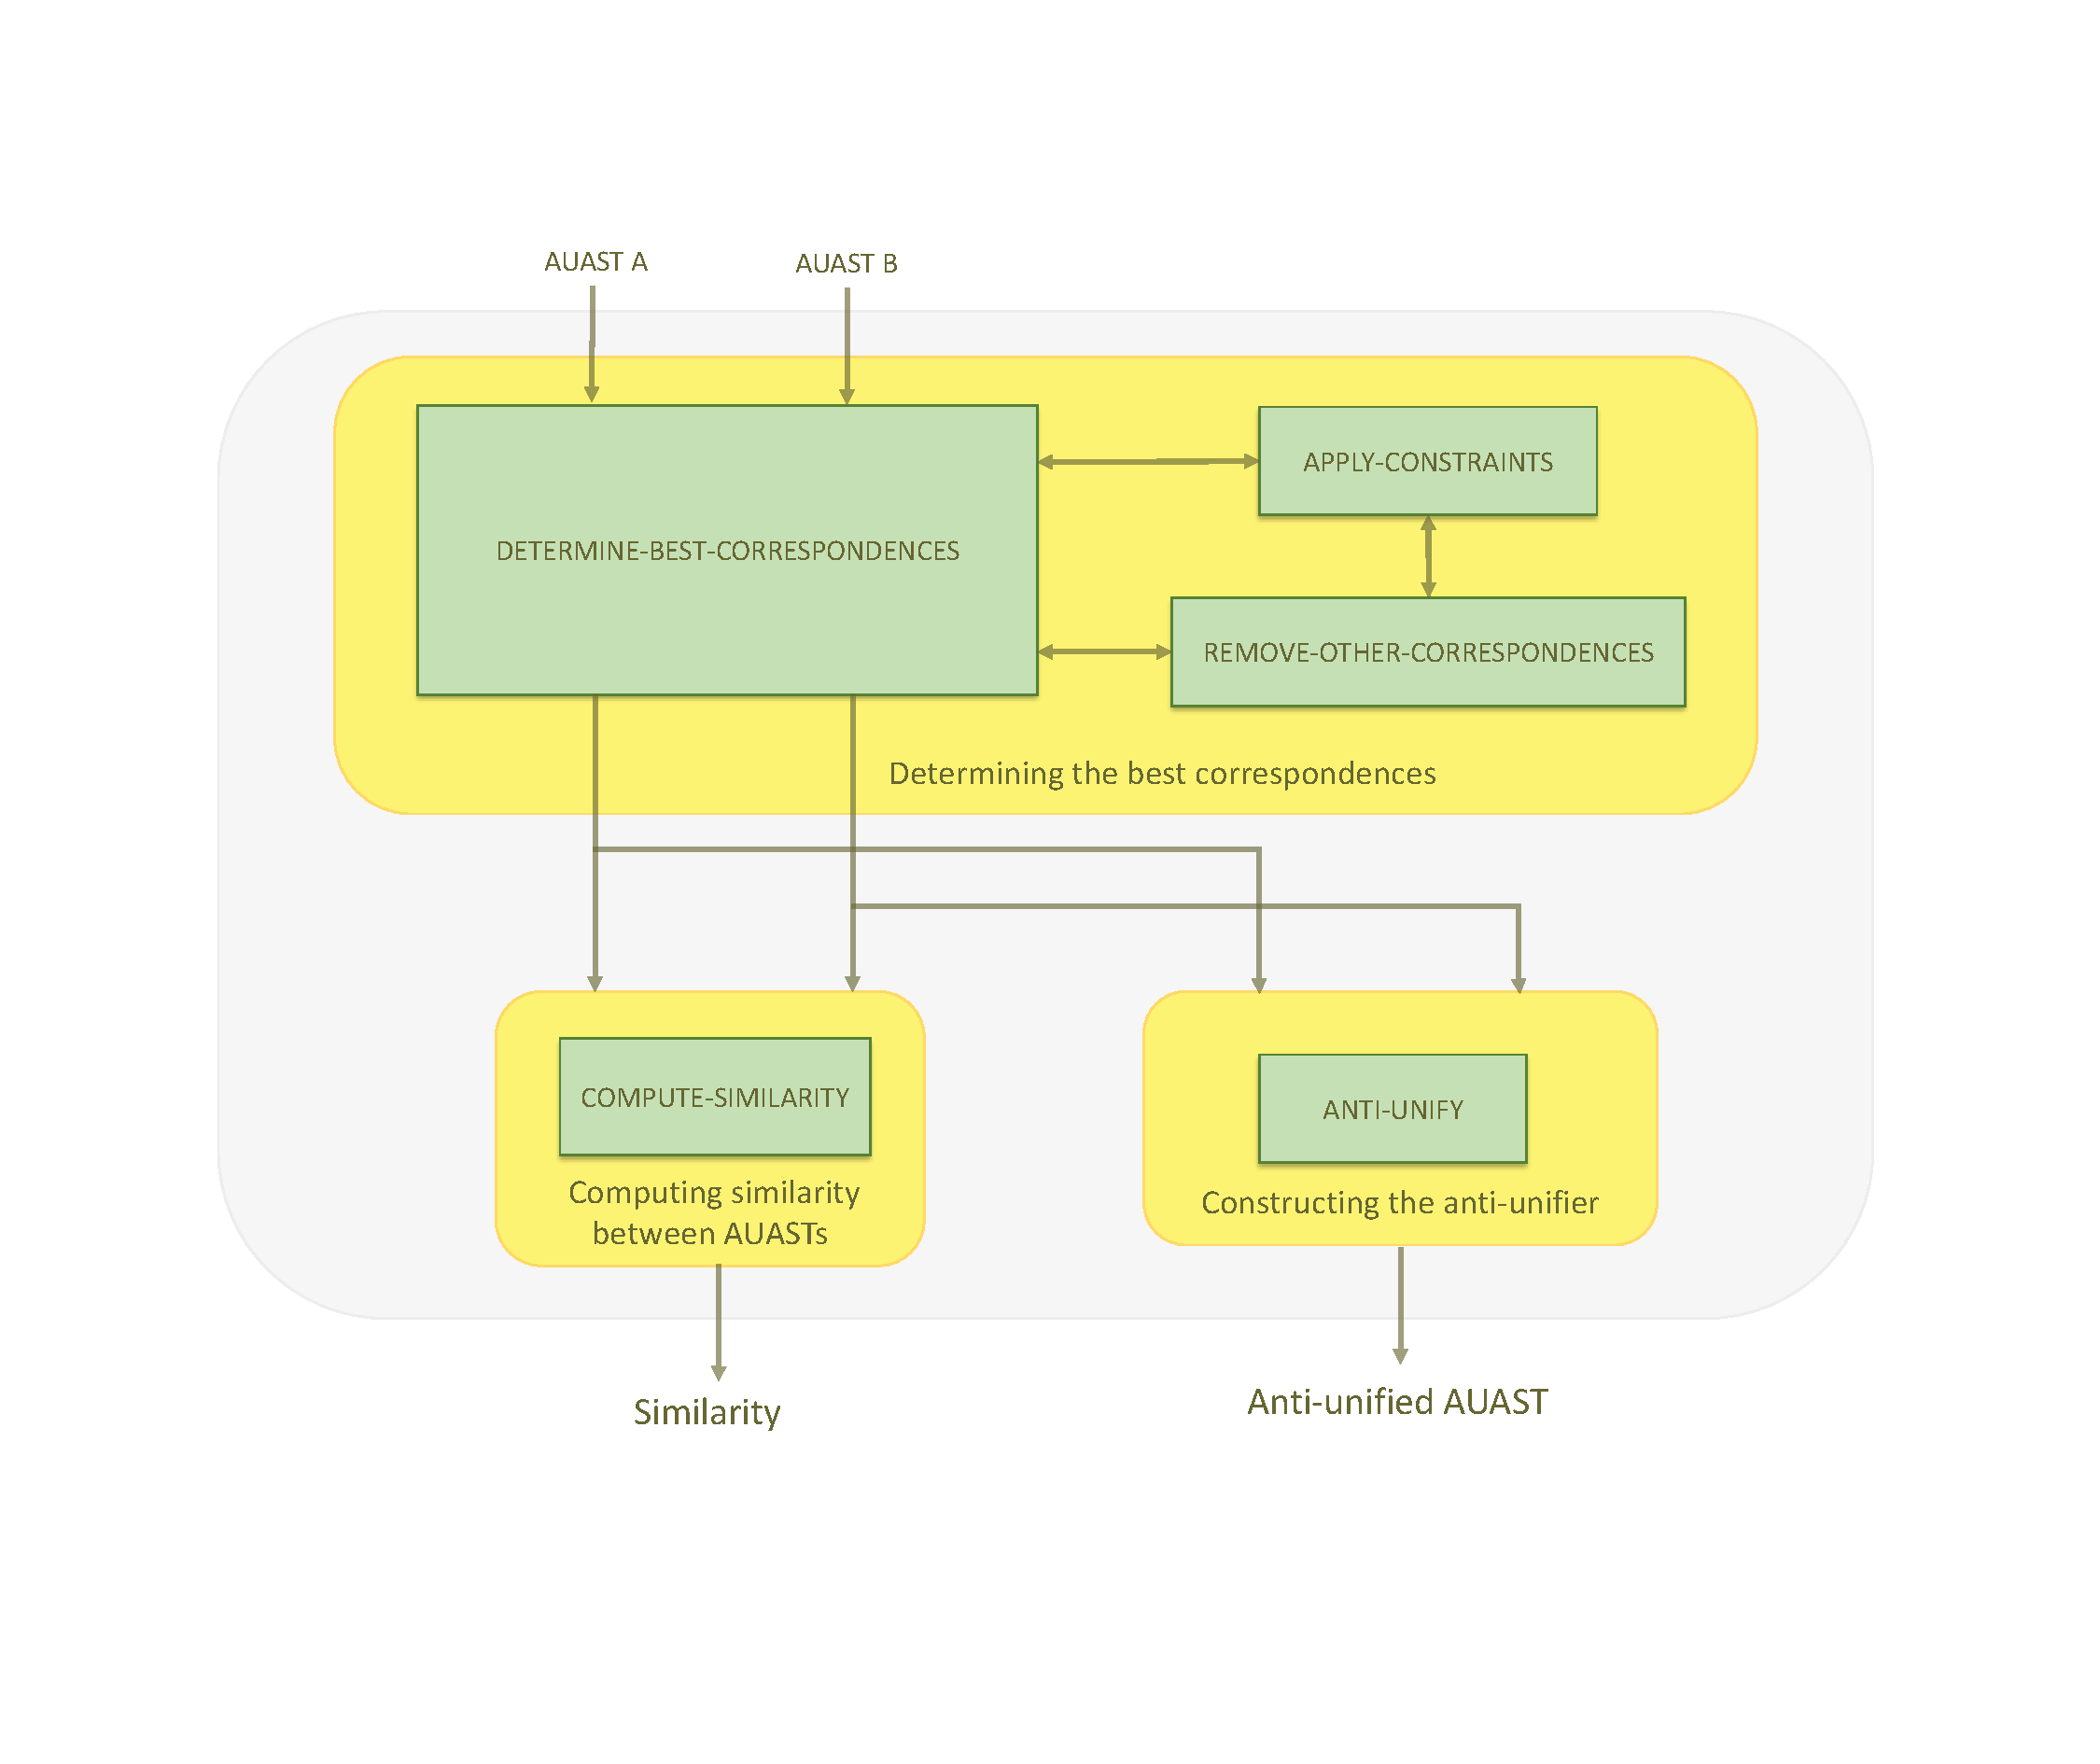
\includegraphics [width = \textwidth]{Drawing4/auOverview.pdf}
  \caption{Overview of the anti-unification process.}
  \label{fig:meth_overview}
\end{figure}


To evaluate my approach, I developed the anti-unifier-building tool atop Jigsaw, and conducted an experimental study on the test suite introduced in Section~\ref{study1_setup}. In Section~\ref{antiunifierTool}, I discuss the algorithms and decisions I made for implementing the anti-unifier-building tool and constructing a detailed view of the structural generalization. I also describe my experimental setup, present the study, and discuss the results in Section~\ref{anti-unifier-assessment}.



%abstracts structural correspondences of ASTs
%A generalization mechanism could be used to abstract commonalities in several structures containing logging calls into a more general structure;
%The higher-order anti-unification modulo theories framework could assist us in constructing a structural generalization from a pair of LCSs. Also, A modified version of a hierarchical clustering suited for our application could assist us to construct a generalization from a set of LMs.

%To construct a structural generalization from a pair of LMs, we developed a prototype tool that applies the Jigsaw framework to find candidate correspondences between two ASTs and uses higher-order anti-unification modulo theories to generalize the structures. It takes the source code of two logged \name{Java} methods as input and performs a sequence of six actions on them, outlined by the algorithm \func{Anti-unification}: (1) we input into the algorithm the ASTs of two given logged \name{Java} methods, constructed via the Eclipse Java Development Tools (JDT) framework; (2) we generate an augmented form of AST (called a CAST) using the Jigsaw framework, where each node holds a list of candidate correspondence connections between the two ASTs (line~1) (see Section~\ref{meth-CAST}); (3) we extend the CAST structure to a higher-order extended structure (called an AUAST) and apply some constraints to prevent the anti-unification of logging calls with anything else (lines~2--3) (see Sections~\ref{meth-constructAUAST} and~\ref{meth-constraints}); (4) we determine the best correspondence for each node of the AUASTs with the highest similarity and we remove the other correspondence connections involving the nodes (line~4) (see Section~\ref{meth-correspondence}); (5) we anti-unify structural properties with their best correspondence to construct an approximation of the best anti-unifier to our problem with special attention to logging calls (line~5) (see Section~\ref{meth-antiUnifier}); and (6) we measure similarity (line~6) (see Section~\ref{meth-similarity}).
%\begin{algorithm}
%\caption{Input into \func{Anti-unification}(\id{auastA},\id{auastB}) are AUAST nodes of two \name{Java} classes containing logging calls; this algorithm construct an anti-unified AUAST node through anti-unification of input node's structural properties} %and compute similarity between them with a focus on logging calls}
%\label{overview}
%\begin{algorithmic}[1]
%\antiunification
%    \State  $\func{Jigsaw-Correspondence}(\id{auastA},\id{auastB})$
%   \State $\id{auastA}, \id{auastB} \gets \func{Apply-Constrains}(\id{auastA},\id{auastB})$
%   \State $$list}  \gets \func{Determine-Best-Correspondences}(\id{auastA})$
%     \State $$compute-similarity} \gets \func{Compute-Similarity}(\id{auastA},\id{auastB})$
%    \State $$anti-unifier} \gets \func{Antiunify}(\id{auastA},\id{auastB})$
%\end{algorithmic}
%\end{algorithm}


%\section{Anti-unification of a pair of ASTs} \label{anti-unification pairs}
%\subsection{Anti-unification ASTs}\label{AUAST}
%\RW{Describe testing/evaluation.}


%\section{Anti-unification ASTs} \label{anti-unification pairs}






\section{Determining the best correspondences}  \label{best-corr}
%As described in Section~\ref{Jigsaw}, through the application of Jigsaw, each AUAST node will hold a list of candidate correspondence connections, each implicitly representing an anti-unifier. However, despite having multiple potential anti-unifiers, we need to determine one single anti-unifier that is helpful to solve our problem using the greedy selection algorithm discussed in Section~\ref{}.


As discussed in Section~\ref{HOAUMT}, the complexity of determining the best anti-unifier is undecidable in general. Therefore, to find one single anti-unifier that is an approximation of the optimal fit to my problem, I developed the \func{Determine-Best-Correspondences} algorithm that greedily selects the most similar correspondence as the best fit for each AUAST node. Therefore, each AUAST node can either be anti-unified with its best correspondence in the other AUAST or with \nothing. This algorithm takes one of the AUASTs, visiting the AUAST nodes therein to store all candidate correspondence connections between the two AUAST nodes in a list, which is sorted in descending order based on the similarity measure (lines~1--9). However, to prevent the anti-unification of log statement nodes with any other nodes, some constraints should be applied on the selection of correspondence connections prior to determining the best ones via the \func{Apply-Constraints} algorithm (Line~8). Then the correspondence connection with the highest similarity value is determined as the best fit for the two nodes involved, and all other correspondence connections involving these nodes are removed using \func{Remove-Other-Correspondences} algorithm (lines~10--14). This process terminates when no more correspondence connections are left in the list.

%entire --> one single

\begin{algorithm}
\caption{\func{Determine-Best-Correspondences}($\id{a}$) takes in the one of the AUASTs and determines the best correspondence connection with the highest similarity for each node.}
\label{alg-determine}
\begin{algorithmic}[1]
\DetermineBest
    \State $\id{list} \gets \func{()}$
    \State $\id{nodes} \gets \func{visitor}(\id{a})$
	  \For {$\id{nodeA} \in \id{a}$}
		\For {$\id{corr} \in  \id{corrs}[\id{nodeA}]$}		
				 	\State{$\func{Append}(\id{corr},\id{list})$ }
			 	\EndFor  	
	   \EndFor	
	    \State{$ \func{Apply-Constraints}(\id{list}) $}	
	   \State{$\func{sort}(\id{list})$}
	   \For{$\id{corr} \in \id{list}$}
	   		\State $\id{bestCorr}[\id{nodeA}] \gets \id{corr}$
	   		\State $\id{bestCorr}[\id{nodeB}] \gets \id{corr}$
	   		\State{$\func{Remove-Other-Correspondences}(\id{corr},\id{list})$ }
	   \EndFor
 %\Return $\id{list} $  	
  \end{algorithmic}
\end{algorithm}

To construct an anti-unifier of the AUASTs of logged methods with a focus on logging calls, some constraints should be applied in determining correspondences. The first constraint (as described below) should be applied to prevent the anti-unification of log statement nodes with any other types of nodes.
\begin{constraint}
A logging call should either be anti-unified with another logging call or should be anti-unified with \nothing.
\end{constraint}	
	
This constraint creates a further constraint:

\begin{constraint}
A structure containing a logging call should be anti-unified with a corresponding structure containing another logging call or should be anti-unified with \nothing.
\end{constraint}

As an illustration consider the CASTs of the two examples in Figure~\ref{fig:meth-ast-1}. As it is shown, there is a candidate correspondence connection between the two log method invocation nodes and the two \code{if} statements. As is clear, the second \code{if} statement contains a logging call, while there is no corresponding logging call in the first one. According to the first constraint, two log method invocation nodes should be anti-unified together. On the other hand, a correspondence connection is created between the two \code{if} statements; however, anti-unification of these statements includes anti-unifying their children nodes as well. Thus, statements inside the body of the \code{if} statements must be anti-unified with each other, indicating that log method invocation inside the body of \code{if} statement in the second example should be anti-unified with \nothing, which is contrary to our first assumption. In order to comply with the first constraint, the correspondence connection between two \code{if} statements should be deleted, leading us to apply the second constraint. My approach applies these constraints by taking the following steps prior to determining the best correspondences:
\begin{enumerate} [leftmargin=.4in]
\item	Augment a property to the AUAST node to mark log statement nodes and structures enclosing them as ``logged''.
\item	Remove correspondence connections where one node is marked as ``logged'' and the corresponding node is not via the \func{Apply-Constraints} algorithm.
\end{enumerate}

The \func{Apply-Constraints} algorithm takes the list of correspondence connections, and removes the ones involving two nodes where one is ``logged'' and the corresponding node is not, using the \func{Remove-Other-Correspondences} algorithm (lines~1--9).

\begin{algorithm}
  \caption{\func{Apply-Constraints}($\id{list}$) applies the constraints on the list of correspondence connections.}
  \label{computeMatches}
  \begin{algorithmic}[1]
  \ApplyConstraints
      \For {$\id{corr} \in \id{list}$}
      \State $\id{nodeA} \gets \id{nodeA}[\id{corr}]$
	  \State $\id{nodeB} \gets \id{nodeB}[\id{corr}]$
 			\If {($\id{nodeA} \Instanceof \cons{Logged}) \And (\id{nodeB} \Instanceof \cons{Non-Logged}$)}	
 		\State{$\func{Remove-Other-Correspondences}(\id{corr},\id{list})$ }
	   	\ElsIf {$(\id{nodeA} \Instanceof \cons{Non-Logged}) \And (\id{nodeB} \Instanceof \cons{Logged}$) }	
  		\State{$\func{Remove-Other-Correspondences}(\id{corr},\id{list})$ }
	  \EndIf 		
 \EndFor 	
	
  \end{algorithmic}
\end{algorithm}




\func{Remove-Other-Correspondences} algorithm removes correspondence connections that are not selected as the best fit from three lists: the list of all correspondence connections (Line~5 and Line~12);
the list of correspondence connections of the first node involved in the connection (Line~6 and Line~13); the list of correspondence connections of the second node involved in the connection (Line~7 and Line~14). As an example, Figure~\ref{fig:AUASTs} shows the correspondence connections between AUAST nodes after applying the \func{Determine-Best-Correspondence} algorithm on the list of potential correspondence connections.
%in Figure~\ref{fig:meth-ast-1}.

\begin{algorithm}
\caption{\func{Remove-Other-Correspondences}($\id{corr}$,$\id{list}$) removes all other correspondences involving the nodes of a particular correspondence connection ($\id{corr}$) from the lists of correspondences.}
\label{removeOtherCEs}
  \begin{algorithmic}[1]
  \RemoveOtherCEs
       \State $\id{listA} \gets \id{corrs}[\id{nodeA}[\id{corr}]]$
	   \State $\id{listB} \gets \id{corrs}[\id{nodeB}[\id{corr}]]$
	   \For {$\id{corrA} \in \id{listA}$}
			\If{$\id{corrA} \neq \id{corr}$}	
\State{$\func{Remove}(\id{corrA},\id{listA})$ } 			
\State{$\func{Remove}(\id{corrA},\id{corrs}[\id{nodeA}[\id{corrA}]])$ }
\State{$\func{Remove}(\id{corrA},\id{corrs}[\id{nodeB}[\id{corrA}]])$ }    		
	   		 \EndIf
	   \EndFor		
       \For {$\id{corrB} \in \id{listB}$}
			\If{$\id{corrB} \neq \id{corr}$}	   		 	 	
	 	 	\State{$\func{Remove}(\id{corrB},\id{listB})$ } 		 \State{$\func{Remove}(\id{corrB},\id{corrs}[\id{nodeA}[\id{corrB}]])$ }
\State{$\func{Remove}(\id{corrB},\id{corrs}[\id{nodeB}[\id{corrB}]])$ }
	   		 \EndIf
	   \EndFor	  	
  \end{algorithmic}
\end{algorithm}




\begin{figure} [H]
  \centering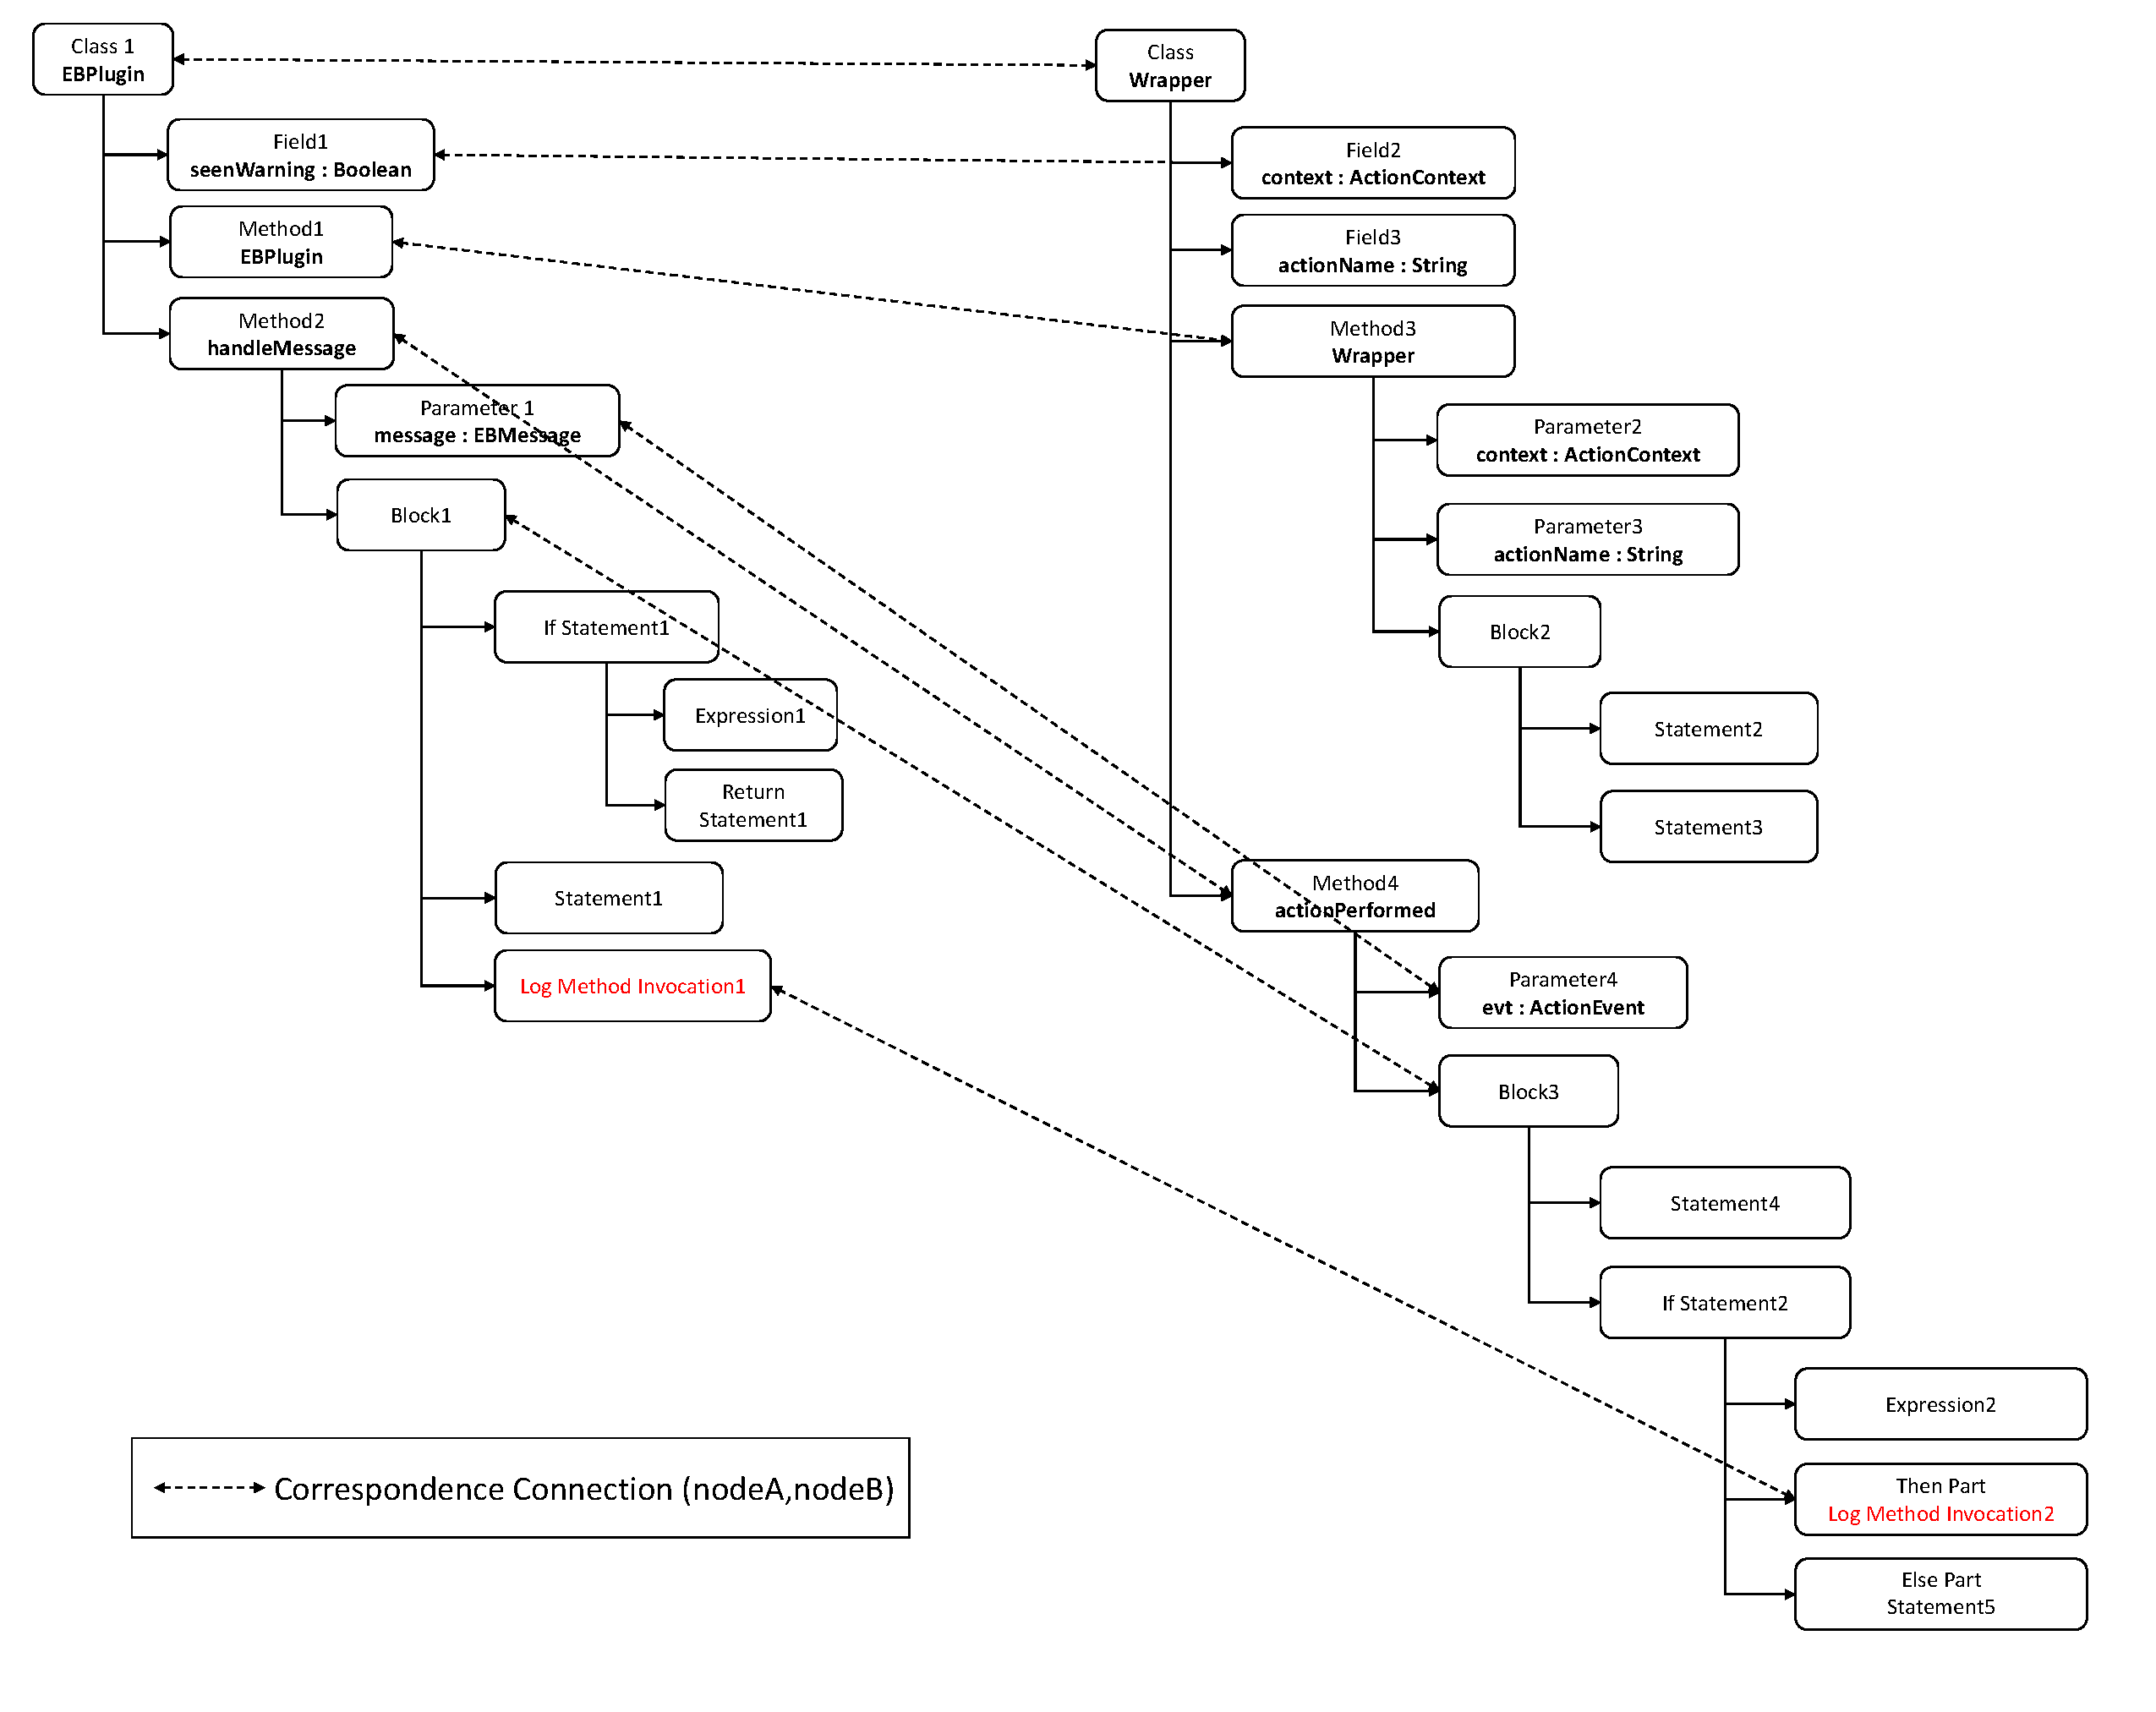
\includegraphics [width = \textwidth]{Drawing4/FinalCorr.pdf}
  \caption{Simple AUAST structure of examples in Figures~\ref{ch3-ex1} and~\ref{ch3-ex2}. The links between AUAST nodes indicate structural correspondences selected as the best fit using the \func{Determine-Best-Correspondences} algorithm.}
  \label{fig:AUASTs}
\end{figure}
%In general, higher order anti-unification modulo theories is undecidable [Cottrell et al., 2008]. That is, the complexity of determining the most optimal MSA is undecidable, but our desire is to create one of the best MSAs to approximate the optimal one that can sufficiently solve our problem, thus the anti-unification process should construct an anti-unifier that is the best approximate fit for our application. To this end, a greedy selection algorithm has been used, which is an approximation technique to determine the best correspondence for each node in the AUAST so constructing the anti-unifier that is approximately the best fit to our problem.

\section{Computing similarity between AUASTs} \label{meth-similarity}
Similarity computation is particularly important for clustering phase that relies on accurate estimation of similarity between logged methods (Chapter~\ref{clustering}). The notion of similarity can differ depending on the given context. That is, similarity between certain features could be highly important for a particular application, while it is not for another. The utility of a similarity function can be determined based on how well it enables us to produce accurate results for a particular task. In this study, a similarity measure is needed to classify logged methods based on the structural similarity in the usage of logging calls. The similarity for my application can be defined as the number of common elements over the total number of elements of the anti-unifier constructed based on the selected correspondences from the previous step.

%computed the ratio of the number of common elements over the total number of elements of the anti-unifier to measure similarity between two AUASTs


% Equation???
% heuristic???

The similarity between two AUAST nodes is computed by dividing the number of matched elements among the two nodes by the size of the largest node (Equation~\ref{eq-jigsaw-sim}). The number of matches between the two AUASTS $\id{a}$ and $\id{b}$ is computed via the \func{Compute-Best-Matches} algorithm. If the two AUASTs are of leaf nodes, the number of matches is computed using the heuristics proposed by \citet{2008:fse:cottrell} (Section~\ref{Jigsaw}) (Lines~2--3). Otherwise, the best correspondences between the two subtrees are selected using the \func{Determine-Best-Correspondences} algorithm, and the matches between each children of the subtree $\id{a}$ and its best corresponding node in the subtree $\id{b}$ is computed and propagated to the parent node (Lines~4--12).


\begin{algorithm}
 \caption{\func{Compute-Best-Matches}($\id{a}$,$\id{b}$) computes the matches between the two ASTs based on the best correspondences.}
  \label{simi}
  \begin{algorithmic}[1]
  \ComputeBestMatches
  \State $\id{matches} \gets 0$
\If {$\id{a} \Instanceof \cons{Leaf-Node}$ }	
  \State $\id{matches} \gets   \func{matches}(\id{a},\id{b})$
  \ElsIf {$\id{a} \Instanceof \cons{Non-Leaf-Node}$ }	
    	\State \func{Determine-Best-Correspondences}($\id{a}$, $\id{b}$)
\For {$\id{childA} \in \id{children}[\id{a}]$}
\If {$ \id{bestCorr}[\id{childA}] \neq \cons{NULL}$}	 		
	%\State $\id{childB}\gets \id{bestCorr}[\id{childA}]$ 		
 		\State $\id{matches} \gets \id{matches}+\func{Compute-Best-Matches}(\id{childA},\id{node}[\id{bestCorr}[\id{childA}]])$		 
 \EndIf
 \EndFor

 \EndIf
 \Return $matches$
\end{algorithmic}
\end{algorithm}



%NIL->0????


%The number of identical structural properties between $\id{auastA}$ and $\id{auastB}$ is computed via the \textsc{Compute-Matches} algorithm through a recursive traversal of $\id{antiunifier}$ nodes' structural properties. For simple structural properties, the number of matches is added by one (Lines~3-4). For child structural properties, the number of matches is added by one and the number of matches computed recursively for the child node (Lines~5-8). For child list structural properties, the number of matches is computed for each child node recursively and is propagated to the parent node (Lines~9-13). All matches are summed up to compute total number of matches between the two AUASTs. Then the following equation is used to compute structural similarity between $\id{auastA}$ and $\id{auastB}$:

\section{Constructing the anti-unifier} \label{meth-antiUnifier}
Once the best correspondences have been determined between two AUASTs, I construct a new anti-unified AUAST by traversing the original AUAST structures recursively and anti-unifying each node with its best correspondence. The new anti-unified structure is a generalization of two original structures, called anti-unifier, where common structural properties are represented by copies and differences are represented by structural variables. The variables may be inserted in place of any node in AUAST, including both subtrees and leaves, and can be substituted with proper original substructures to regain original structures.


% anti-unify the same type nodes????????

Anti-unification of two AUASTs is performed via the \func{Antiunify} algorithm. If the two AUASTs are of leaf nodes, the anti-unifier will be created through the anti-unification of the two nodes (Lines~2--3). Otherwise, the anti-unified subtree is created by anti-unifying each children of one subtree with its best corresponding node in the other subtree. If there is no correspondence for a node, the anti-unified node will be created through the anti-unification of the node with the \NIL{} structure. All these anti-unified nodes are appended to the list of children of the anti-unifier (Lines~4--21). The details of constructing a detailed view of the anti-unifier for my application will be discussed in Section~\ref{meth-detailed-view}.


\begin{algorithm}
 \caption{\func{Antiunify}($\id{a}$,$\id{b}$) creates the anti-unifier of two AUASTs through the anti-unification of each node with its best correspondence.}
  \label{AntiUnify}
  \begin{algorithmic}[1]
\AntiUnify
\State{$ \id{antiunifier} \gets \cons{Null}$}
\If {$\id{a} \Instanceof \cons{Leaf-Node}$ }	
  \State $\id{antiunifier} \gets   \func{construct-antiunifier}(\id{a},\id{b})$
  \ElsIf {$\id{a} \Instanceof \cons{Non-Leaf-Node}$ }	
 % \State \func{Determine-Best-Correspondences}($\id{a}$, $\id{b}$)
        \For {$\id{childA} \in \id{children}[\id{a}]$}
\If {$ bestCorr[childA]= \cons{NULL}$}	
  \State $\id{child} \gets   \func{Antiunify}(\id{childA},\cons{NIL})$
\Else	
 \State $\id{child} \gets   \func{Antiunify}(\id{childA},\id{node}[bestCorr[childA]])$
\EndIf
\State $\func{Append}(\id{child},\id{children[antiunifier]})$
\EndFor
%	\EndIf	
  %\If {$\id{b} \Instanceof \cons{Non-Leaf-Node}$ }	
\EndIf
  \If {$\id{b} \Instanceof \cons{Non-Leaf-Node}$ }	

  \For {$\id{childB} \in \id{children}[\id{b}]$}
\If {$ bestCorr[childB]= \cons{NULL}$}	
  \State $\id{child} \gets   \func{Antiunify}(\id{childB},\cons{NIL})$
\EndIf
\State $\func{Append}(\id{child},\id{children[antiunifier]})$
\EndFor
 \EndIf
\Return $\id{antiunifier}$
\end{algorithmic}
\end{algorithm}



\section{The Anti-unifier building tool} \label{antiunifierTool}
The anti-unifier building tool is a proof-of-concept implementation of my anti-unification approach, which is developed atop the Jigsaw framework to construct a detailed view of structural generalization. To create the AUAST structure using Eclipse JDT framework that addresses the limitations of CAST to constructing an anti-unifier, I added the following structural properties:
%namely?
%to address the limitations of CAST to constructing an anti-unifier
%It also creates an extended form of CAST, called AUAST,
\begin{itemize} [leftmargin=.5in]
\item \textit{Simple structural variable Properties}: an extension of simple structural properties referring to two simple values to allow the insertion of variables in place of leaves.
\end{itemize}
\begin{itemize} [leftmargin=.5in]
\item \textit{Child structural variable properties}: an extension of child structural properties referring to two child AST nodes to allow the insertion of variables in place of subtrees.
\end{itemize}

I also needed to make additional algorithms and decisions to construct a detailed generalization view suited to my application, which will be described in the following sections.

%%change???


\subsection{Constructing the detailed generalization view} \label{meth-detailed-view}

To figure out the structural commonalities and differences amongst logged methods, I developed an algorithm to construct a generalization view of the anti-unifier. Figure~\ref{fig:meth-anti-unifier} shows a simple detailed view I used to represent the anti-unifier constructed from the AUASTs of logged methods of Examples 1 and 2, where ``$\id{a}$-or-$\id{b}$'' represents a structural variable that must be substituted with either the $a$ or $b$ substructures to recover each original structure, and ``$\id{a}$'' represents that the $a$ substructure is common between the two AUASTs.
%??????


% modify the figure???

\begin{figure} [H]
  \centering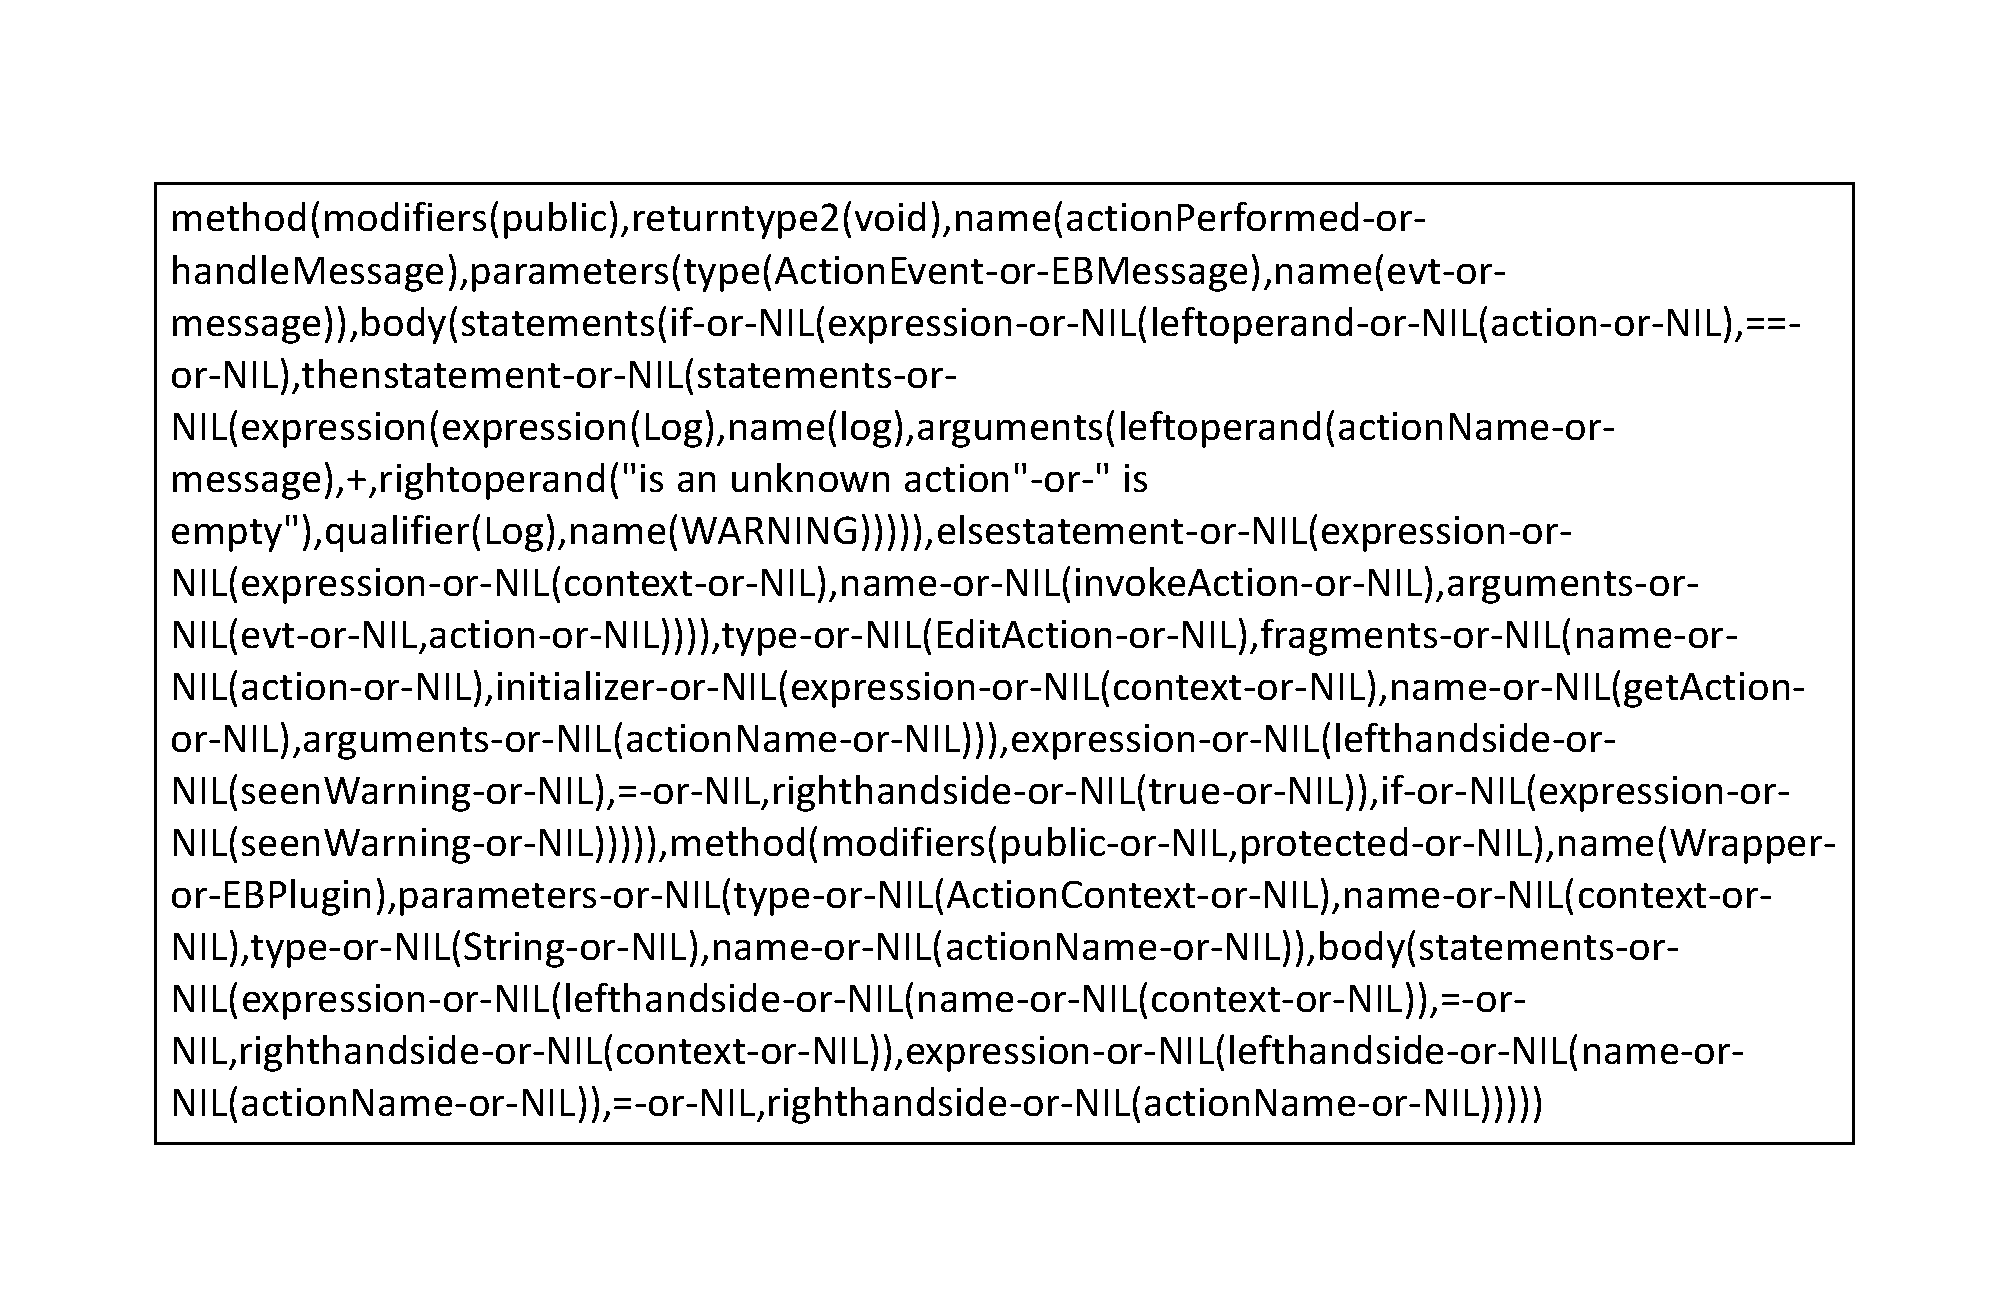
\includegraphics [scale=0.5]{Drawing4/auMethod.pdf}
  \caption{Simple detailed view of the anti-unifier constructed from the AUASTs of Examples 1 and 2.}
  \label{fig:meth-anti-unifier}
\end{figure}

% the LMs in
% to create an anti-unifier description. For example, we supply the \func{Antiunify} algorithm with the AUASTs of LMs in Examples 1 and 2
%explain in more details???

To create the detailed view of the structural generalization from two given AUASTs, I applied the \func{Antiunify} algorithm presented in Section~\ref{meth-antiUnifier} on the two AUAST nodes $\id{a}$ and $\id{b}$ through the anti-unification of their structural properties, as the Eclipse JDT utilizes these properties to record structural information of each \name{Java} element (Section~ref{JDT}). That is, for each structural property of the two nodes, if the property is common between them, a copy of it will be created and added to the structural properties of the anti-unifier; otherwise, a variable structural property is constructed referring to two property values and and added to the anti-unifier's structural properties.
%property values???


% (Lines~8--9); if structural property is a child property, a child variable structure is constructed (Lines~10--12). All these strcutural prperties will be added to the structural property of the anti-unifier(Lines~8--9). 


%if structural property is a child list property, for each child of $\id{propA}$ and $\id{propB}$, where there is no correspondence in the other AUAST, an anti-unified node is created through the anti-unification of the child node with the \NIL{} structure via the \func{Antiunify} algorithm and added to the value of the anti-unified child list property; otherwise, the child node is anti-unified with its best correspondence (Lines~6-21).


\subsection{Java methods containing multiple logging calls} \label{meth-multipleLogs}
There might be some cases in which our approach is not able to anti-unify logging calls in two input seeds, when there is more than one logging call in a LJM. For example, consider the LMs in Figures~\ref{multiple1} and~\ref{multiple2}. Figure~\ref{mast_1} shows the simple AUASTs for these examples and potential correspondence connections between the AUAST nodes. Figure~\ref{m_ast2} shows the correspondence connections selected as the best match using our greedy algorithm. To anti-unify \code{if statement 1} with \code{if statement 3}, we should anti-unify their structural properties. Thus, \code{log1} should be anti-unified with \code{log3}, and \code{log4} should be anti-unified with \NIL{} since there is no corresponding logging call in the body of \code{if statement 1}, while there is a corresponding logging call for \code{log4} in the body of \code{if statement 2} (\code{log2}).

%\code{if statement 1}???
%In figures: If statement: if statement 1???

\begin{figure}[H]
\def\baselinestretch{1}
\begin{lstlisting}
public void method1(){
	...
	if(condition1){
		Log.log();
	}
	...
	if(condition2){
		Log.log();
	}
	...
}
\end{lstlisting}
\caption{A \name{Java} method that utilizes multiple logging calls.\label{multiple1}}
\end{figure}



\begin{figure}[H]
\def\baselinestretch{1}
\begin{lstlisting}
public void method2(){
	...
	if(condition3){
		Log.log();
		Log.log();
	}
	...
}
\end{lstlisting}
\caption{A \name{Java} method that utilizes multiple logging calls.\label{multiple2}}
\end{figure}

\begin{figure} [H]
  \centering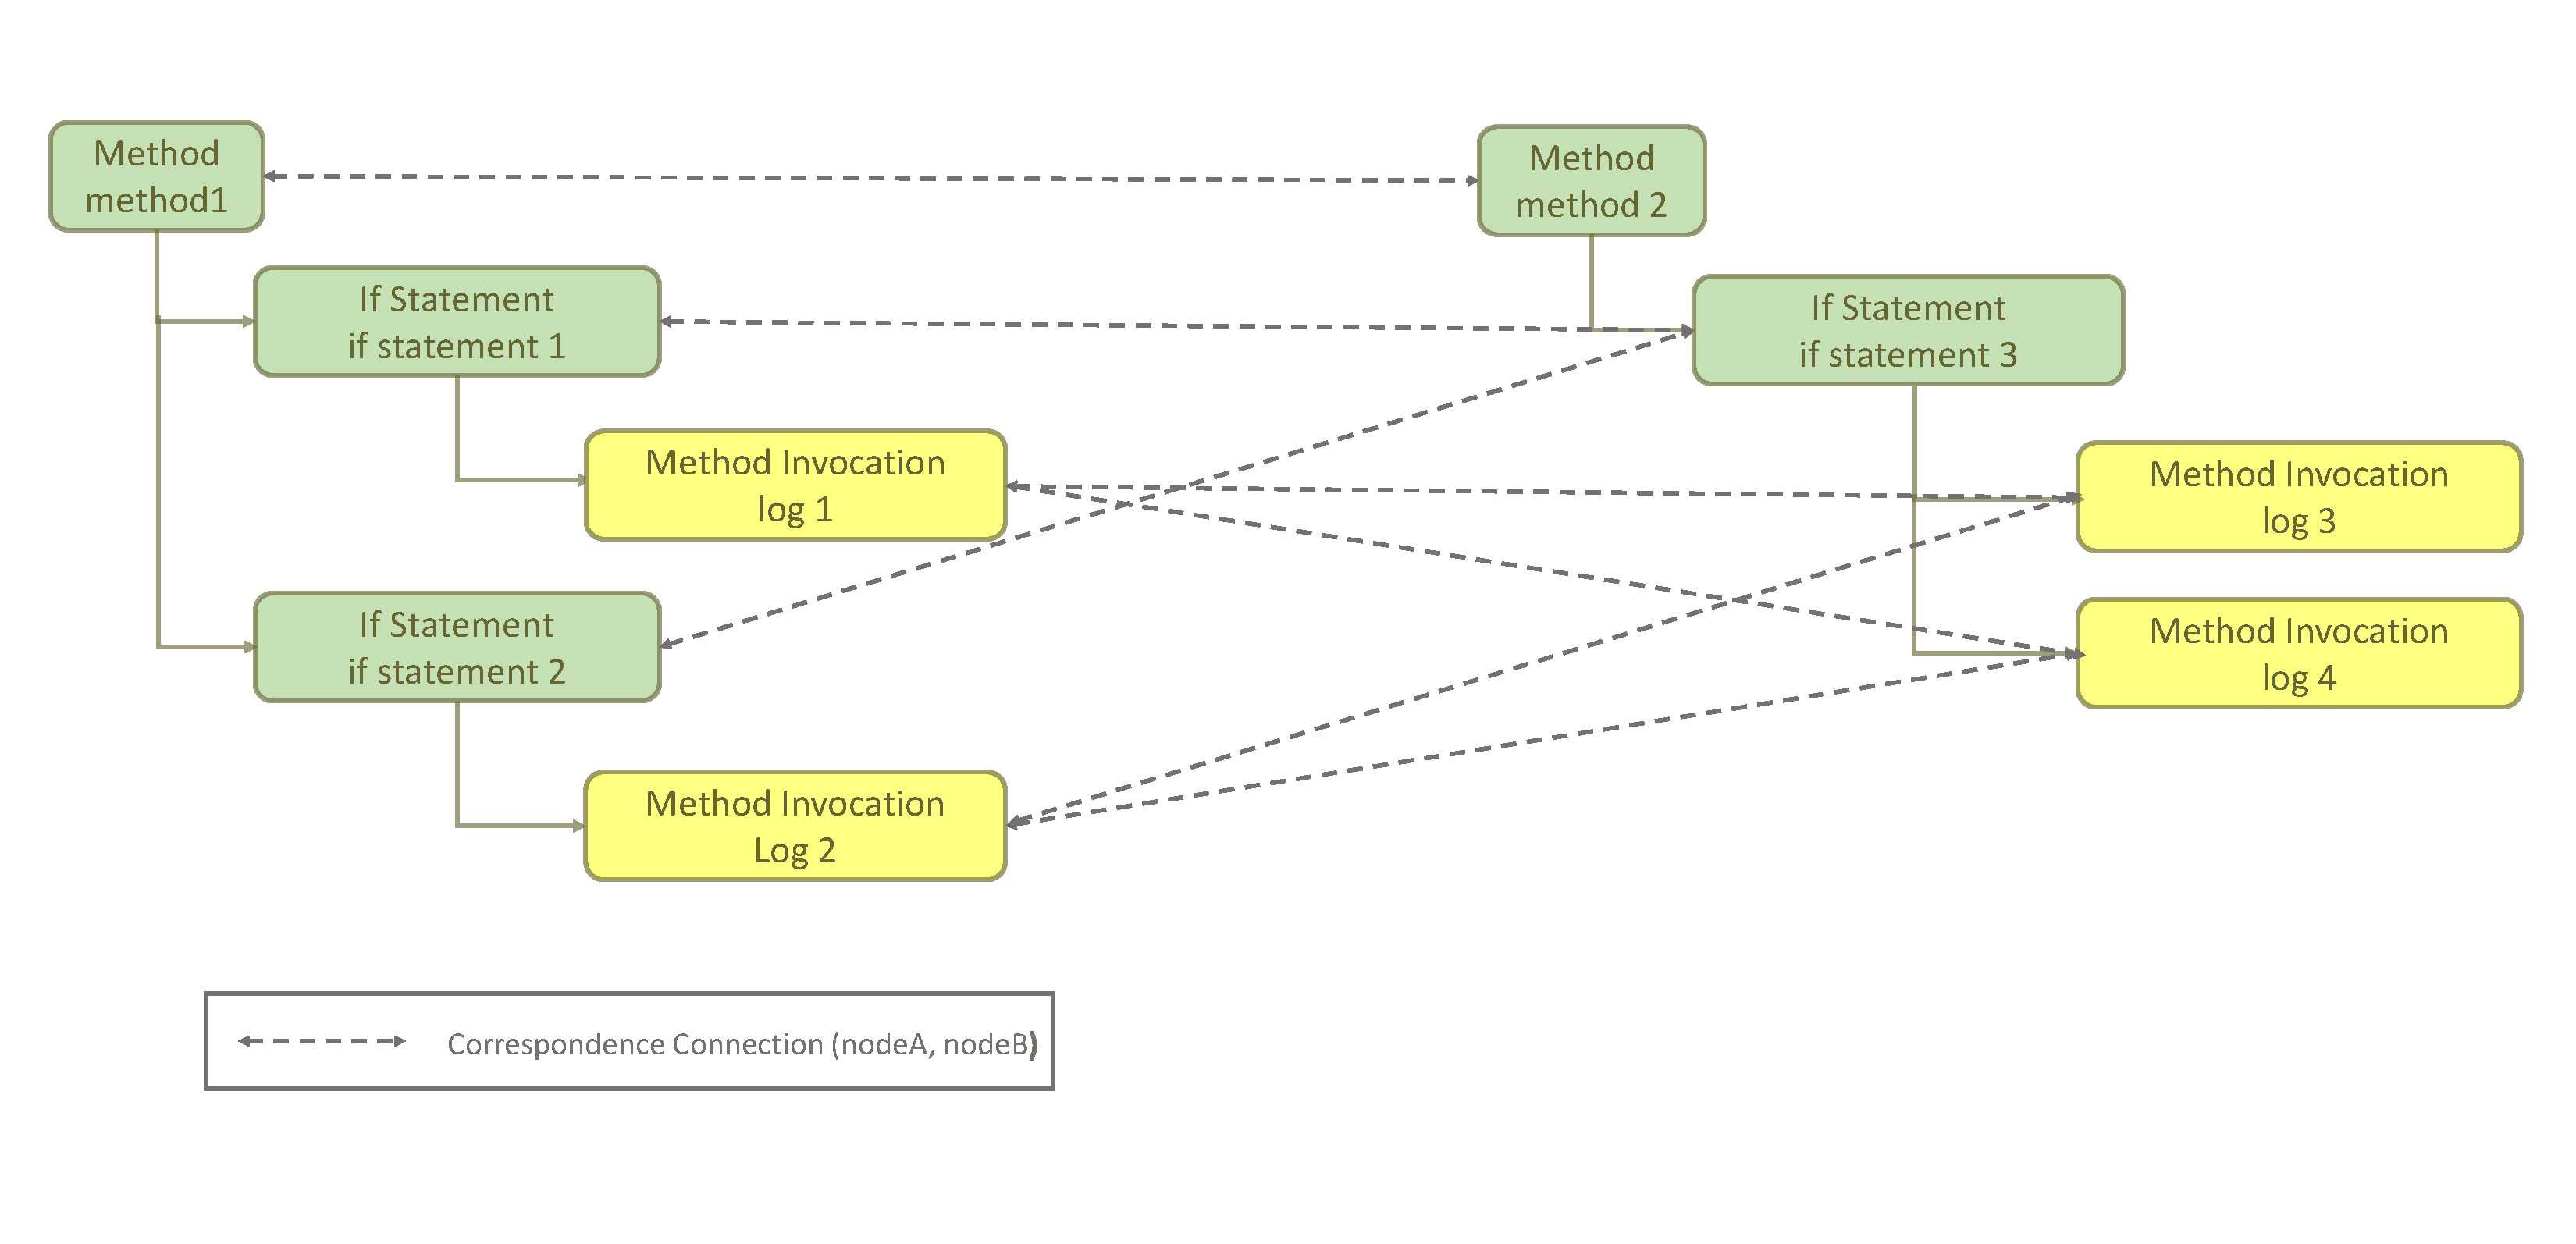
\includegraphics [width = \textwidth]{Drawing4/multipleLogging.pdf}
  \caption{Simple AUAST structure of examples in Figures~\ref{multiple1} and~\ref{multiple2}. Links between AUAST nodes indicate candidate structural correspondences detected by the Jigsaw framework.}
  \label{mast_1}
\end{figure}


\begin{figure} [H]
  \centering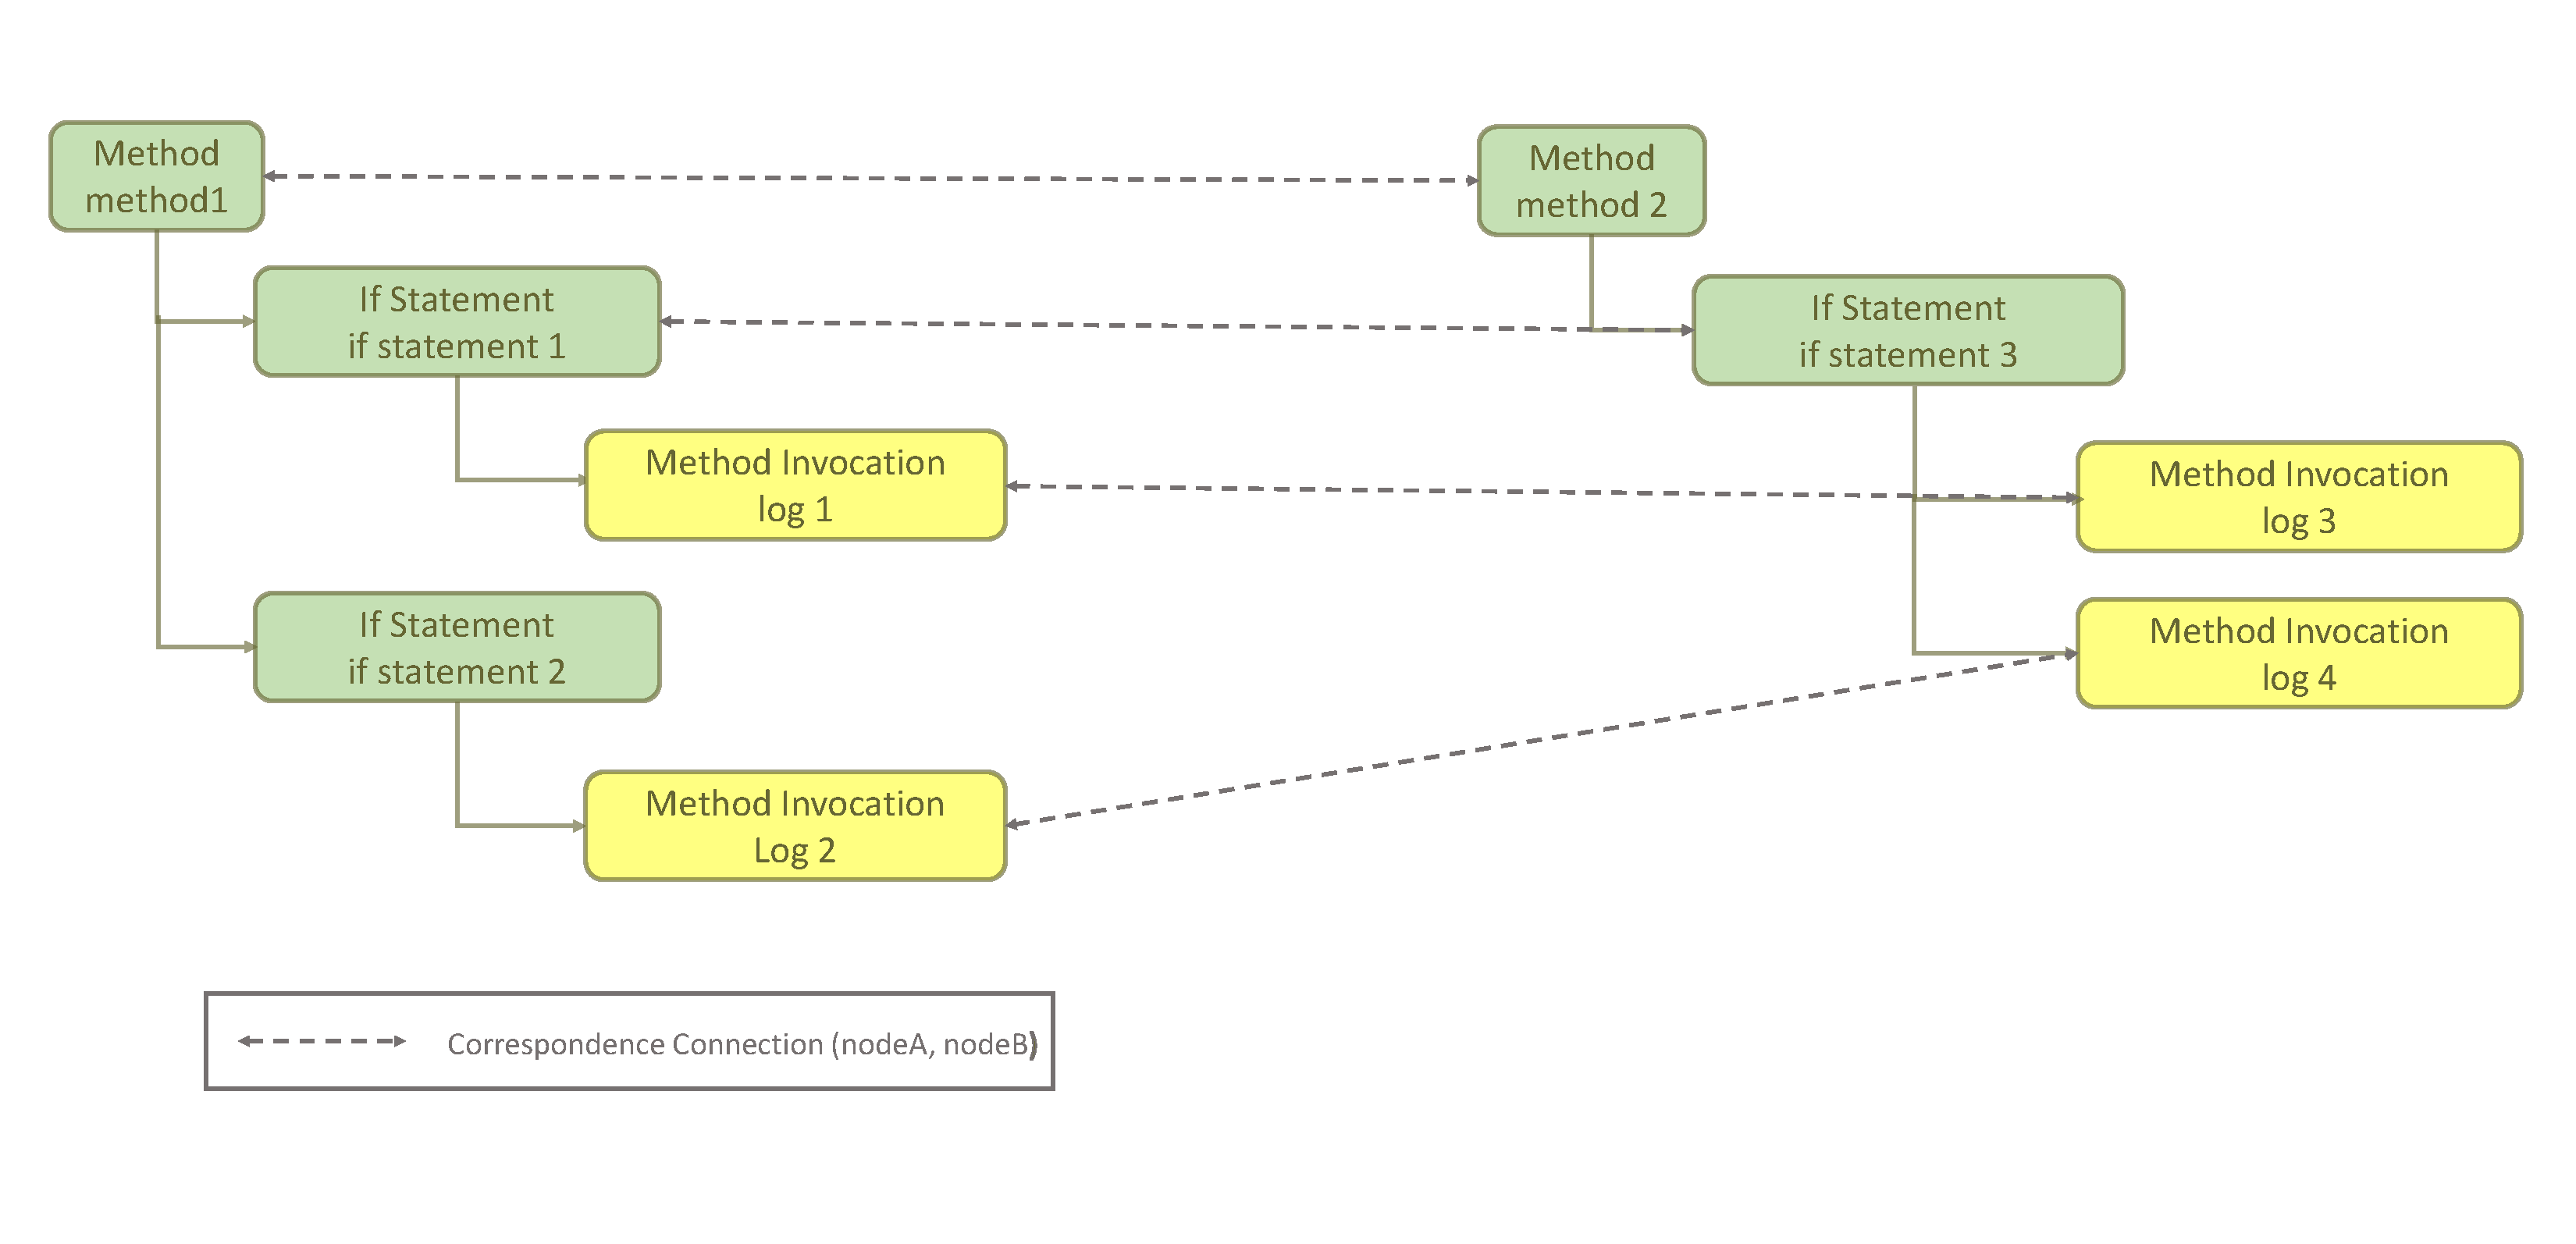
\includegraphics [width = \textwidth]{Drawing4/multipleLogging2.pdf}
  \caption{Simple AUAST structure of examples in Figures~\ref{multiple1} and~\ref{multiple2}. Links between AUAST nodes indicate structural correspondences selected as the best match using our greedy algorithm.}
  \label{m_ast2}
\end{figure}

To handle these cases, we can split them into more than one case, where each LJM contains only one logging call. To do so, we need to create a copy of LJM for each logging call by maintaining that logging call and removing the other ones. For example, we need to create two copies for each logged \name{Java} method of examples in Figures~\ref{multiple1} and~\ref{multiple2} as depicted in Figures~\ref{multiple1-one} and~\ref{multiple2-one}, respectively.
% thus constructing four possible anti-unifier for  possible combination and compute the similarity for each combination.
%We can split this case into more than one case, each with one logging statement in every seed. That is, for each case all the other logging statements should be deleted from seeds.  For example, imagine we have AST 1 and AST 2. AST 1 contains three logging calls and AST 2 contains two logging calls. As explained, we split AST 1 into AST 1a, AST 1b, and AST 1c. Also, we split AST 2 into AST 2a and AST 2b. We can split this case into 6 possible cases and create an anti-unifier for each possible combination and then compute a measure of similarity for each case. The best match for each log statement can be selected based on anti-unifier with the highest similarity amongst the other options.


\begin{figure}[H]
\def\baselinestretch{1}
\begin{lstlisting}

public void method1(){
	...
	if(condition1){
		Log.log();
	}
	...
	if(condition2){
		//removed
	}
	...
}

public void method1(){
	...
	if(condition1){
		//removed
	}
	...
	if(condition2){
		Log.log();
	}
	...
}

\end{lstlisting}
\caption{Create multiple copies of the LJM in Figure~\ref{multiple1} for each logging call.\label{multiple1-one}}
\end{figure}



\begin{figure}[H]
\def\baselinestretch{1}
\begin{lstlisting}
public void method2(){
	...
	if(condition3){
		//removed
		Log.log();
	}
	...
}

public void method2(){
	...
	if(condition3){
		Log.log();
		//removed
	}
	...
}

\end{lstlisting}
\caption{Create multiple copies of the LJM in Figure~\ref{multiple2} for each logging call.\label{multiple2-one}}
\end{figure}

%\section{An assessment of the anti-unifier-building tool}\label{anti-unifier-assessment}

\section{Evaluation} \label{anti-unifier-assessment}
%\subsection{Study 2: Detailed anti-unifier view}  \label{study2}
To assess the effectiveness of my anti-unification algorithm and the supporting tool, I conducted an experiment on the test suite described in Section~\ref{study1_setup}. %The anti-unifier-building tool is developed atop the correspondence tool to construct an anti-unifier from AUASTs of each LJM pair in our test suite.


\subsection{Setup}  \label{study2-setup}
In this study, we manually attempted to create the detailed anti-unifier view for each pair of LMs in the test suite (55 test cases in total). We first identified corresponding and non-corresponding \name{Java} elements for each LJM pair with a focus on preventing the correspondence of logging calls with anything else and then represented the anti-unifier in the detailed view (i.e., formatted as in Figure~\ref{fig:meth-anti-unifier}). We also computed the ratio of common \name{Java} elements in the detailed anti-unifier view to total number of \name{Java} elements of the two LMs to measure the similarity.
We also ran the anti-unifier-building tool on each pair of LMs to construct the detailed anti-unifier view for each pair with special attention to logging calls and to measure the similarity between the two LMs. Furthermore, we used \name{EclEmma}, which is a \name{Java} code coverage tool for \name{Eclipse}, to measure the test coverage. Test coverage is defined as a measure of the completeness of the set of test cases.


\begin{figure}
  \centering
  \begin{tabular}{cl}
    \toprule
    Test case & Logged methods \\
    \midrule

    \multirow{2}{*}{{1}}&\code{PluginJAR.generateCache()}\\
                         &\code{PluginJAR.generateCache()}\\
    \midrule

    \multirow{2}{*}{2}&\code{PluginJAR.generateCache()}\\
                         &\code{EditBus.send(..)}*\\
    \midrule

    \multirow{2}{*}{3}&\code{MiscUtilities.isSupportedEncoding(..)}\\
                         &\code{EditBus.send(..)}\\
    \midrule

    \multirow{2}{*}{4}&\code{EditBus.send(..)}\\
                         &\code{EditBus.send(..)}*\\
    \midrule
    \multirow{2}{*}{5}&\code{EditBus.send(..)}*\\
                         &\code{EditAction.Wrapper.actionPerformed(..)}\\
    \midrule

    \multirow{2}{*}{6}&\code{EditBus.send(..)}*\\
                         &\code{BufferHistory.RecentHandler.doctypeDecl(..)}\\
    \midrule

    \multirow{2}{*}{7}&\code{EditAction.Wrapper.actionPerformed(..)}\\
                         &\code{JARClassLoader.loadClass(..)}\\
    \midrule

    \multirow{2}{*}{8}&\code{EditAction.Wrapper.actionPerformed(..)}\\
                         &\code{VFS.DirectoryEntry.RootsEntry.rootEntry(..)}\\
    \midrule

    \multirow{2}{*}{9}&\code{PluginJAR.generateCache()}\\
                         &\code{BufferHistory.RecentHandler.doctypeDecl(..)}\\
    \midrule

    \multirow{2}{*}{10}&\code{VFS.DirectoryEntry.RootsEntry.rootEntry(..)}\\
                         &\code{ServiceManager.loadServices(..)}\\
    \bottomrule

  \end{tabular}
  \caption{10 sample logged \name{Java} method pairs used as test cases; all are contained in the \protect\name{org.gjt.sp.jedit} package with the exception of cases 8 and 10 that are in the \protect\name{org.gjt.sp.jedit.io} package.}
  \label{study2_test_cases}
\end{figure}





%The view would be in the form depicted in ..

\subsection{Results}  \label{study2-results}
We present the results of our analysis for a subset of 10 test cases (see Table~\ref{study2_test_cases}) in Table~\ref{study2_test_cases_results}. The analysis of the output has been divided into two categories: correspondence and similarity. "Correspondence" refers to the number of corresponding lines-of-code (LOC) detected by our tool that were found to be corresponded by our manual examination as well, and the number of LOC detected as corresponded by our tool but were not found to be corresponded in our manual inspection. We also present the percentage of the correct corresponding LOC to the total number of LOC of the two LMs. "Similarity" refers to the similarity that is computed based on the the detected correspondences. It is calculated using both our tool and manual experiment.



In case 8, the \code{rootEntry(..)} method contains a nested \code{if}-statement enclosing a logging call and the \code{actionPerformed(..)} method contains an \code{if}-statement enclosing another logging call. The analysis showed that a correct correspondence was detected between the inner \code{if}-statement inside the nested \code{if}- and the single \code{if}-statement. Cases~3 and~10 contain statements that are not found to correspond by our tool even though correspondences exist. For example, in case 3, the \code{isSupportedEncoding(..)} method contains an assignment statement enclosed by an \code{if}-statement that does not have any correspondences and the \code{send(..)} method contains another assignment statement inside a \code{for}-statement without any correspondences as well. However, no correspondence was detected between the two assignment statements since their parent nodes do not correspond.
\begin{figure}
  \centering
  \begin{tabular}{|c|c|c|c|c|c|}
    \hline
    \multirow{2}{*}{Test case}&\multicolumn{2}{c|}{Correspondence}&\multicolumn{2}{c|}{Similarity}\\
    \cline{2-5}
    &Correct (\%)&Incorrect&human&tool\\
    \hline
    1&104(100)&0& 1.0 & 1.0\\
    \hline
    2&8(100)&0& 0.13& 0.13\\
    \hline
    3&6(85)&1&0.19& 0.16\\
    \hline
    4&4(100)&0&0.29 &0.29\\
    \hline
    5&5(100)&0&0.21 &0.21\\
    \hline
    6&3(100)&0&0.2 &0.2\\
    \hline
    7&5(100)&0&0.11 &0.11\\
    \hline
    8&7(100)&0& 0.1&0.1\\
    \hline
    9&3(100)&0&0.03&0.03 \\
    \hline
    10&14(87)&2&0.27 &0.22\\
    \hline

  \end{tabular}
  \caption{Results of constructing anti-unifiers with a focus on logging calls for the 55 test cases.}

  \label{study2_test_cases_results}
\end{figure}

The results of the pairwise comparison between LMs of the test suite is visualized in Figure~\ref{fig:au_graph}. Our anti-unifier-building tool succeeded in detecting correspondences with special attention to anti-unifying logging calls and calculating pairwise similarities in 48 out of 55 test cases. In addition, the test coverage of our test cases was measured 82\% using \name{EclEmma}.

\begin{figure} [H]
  \centering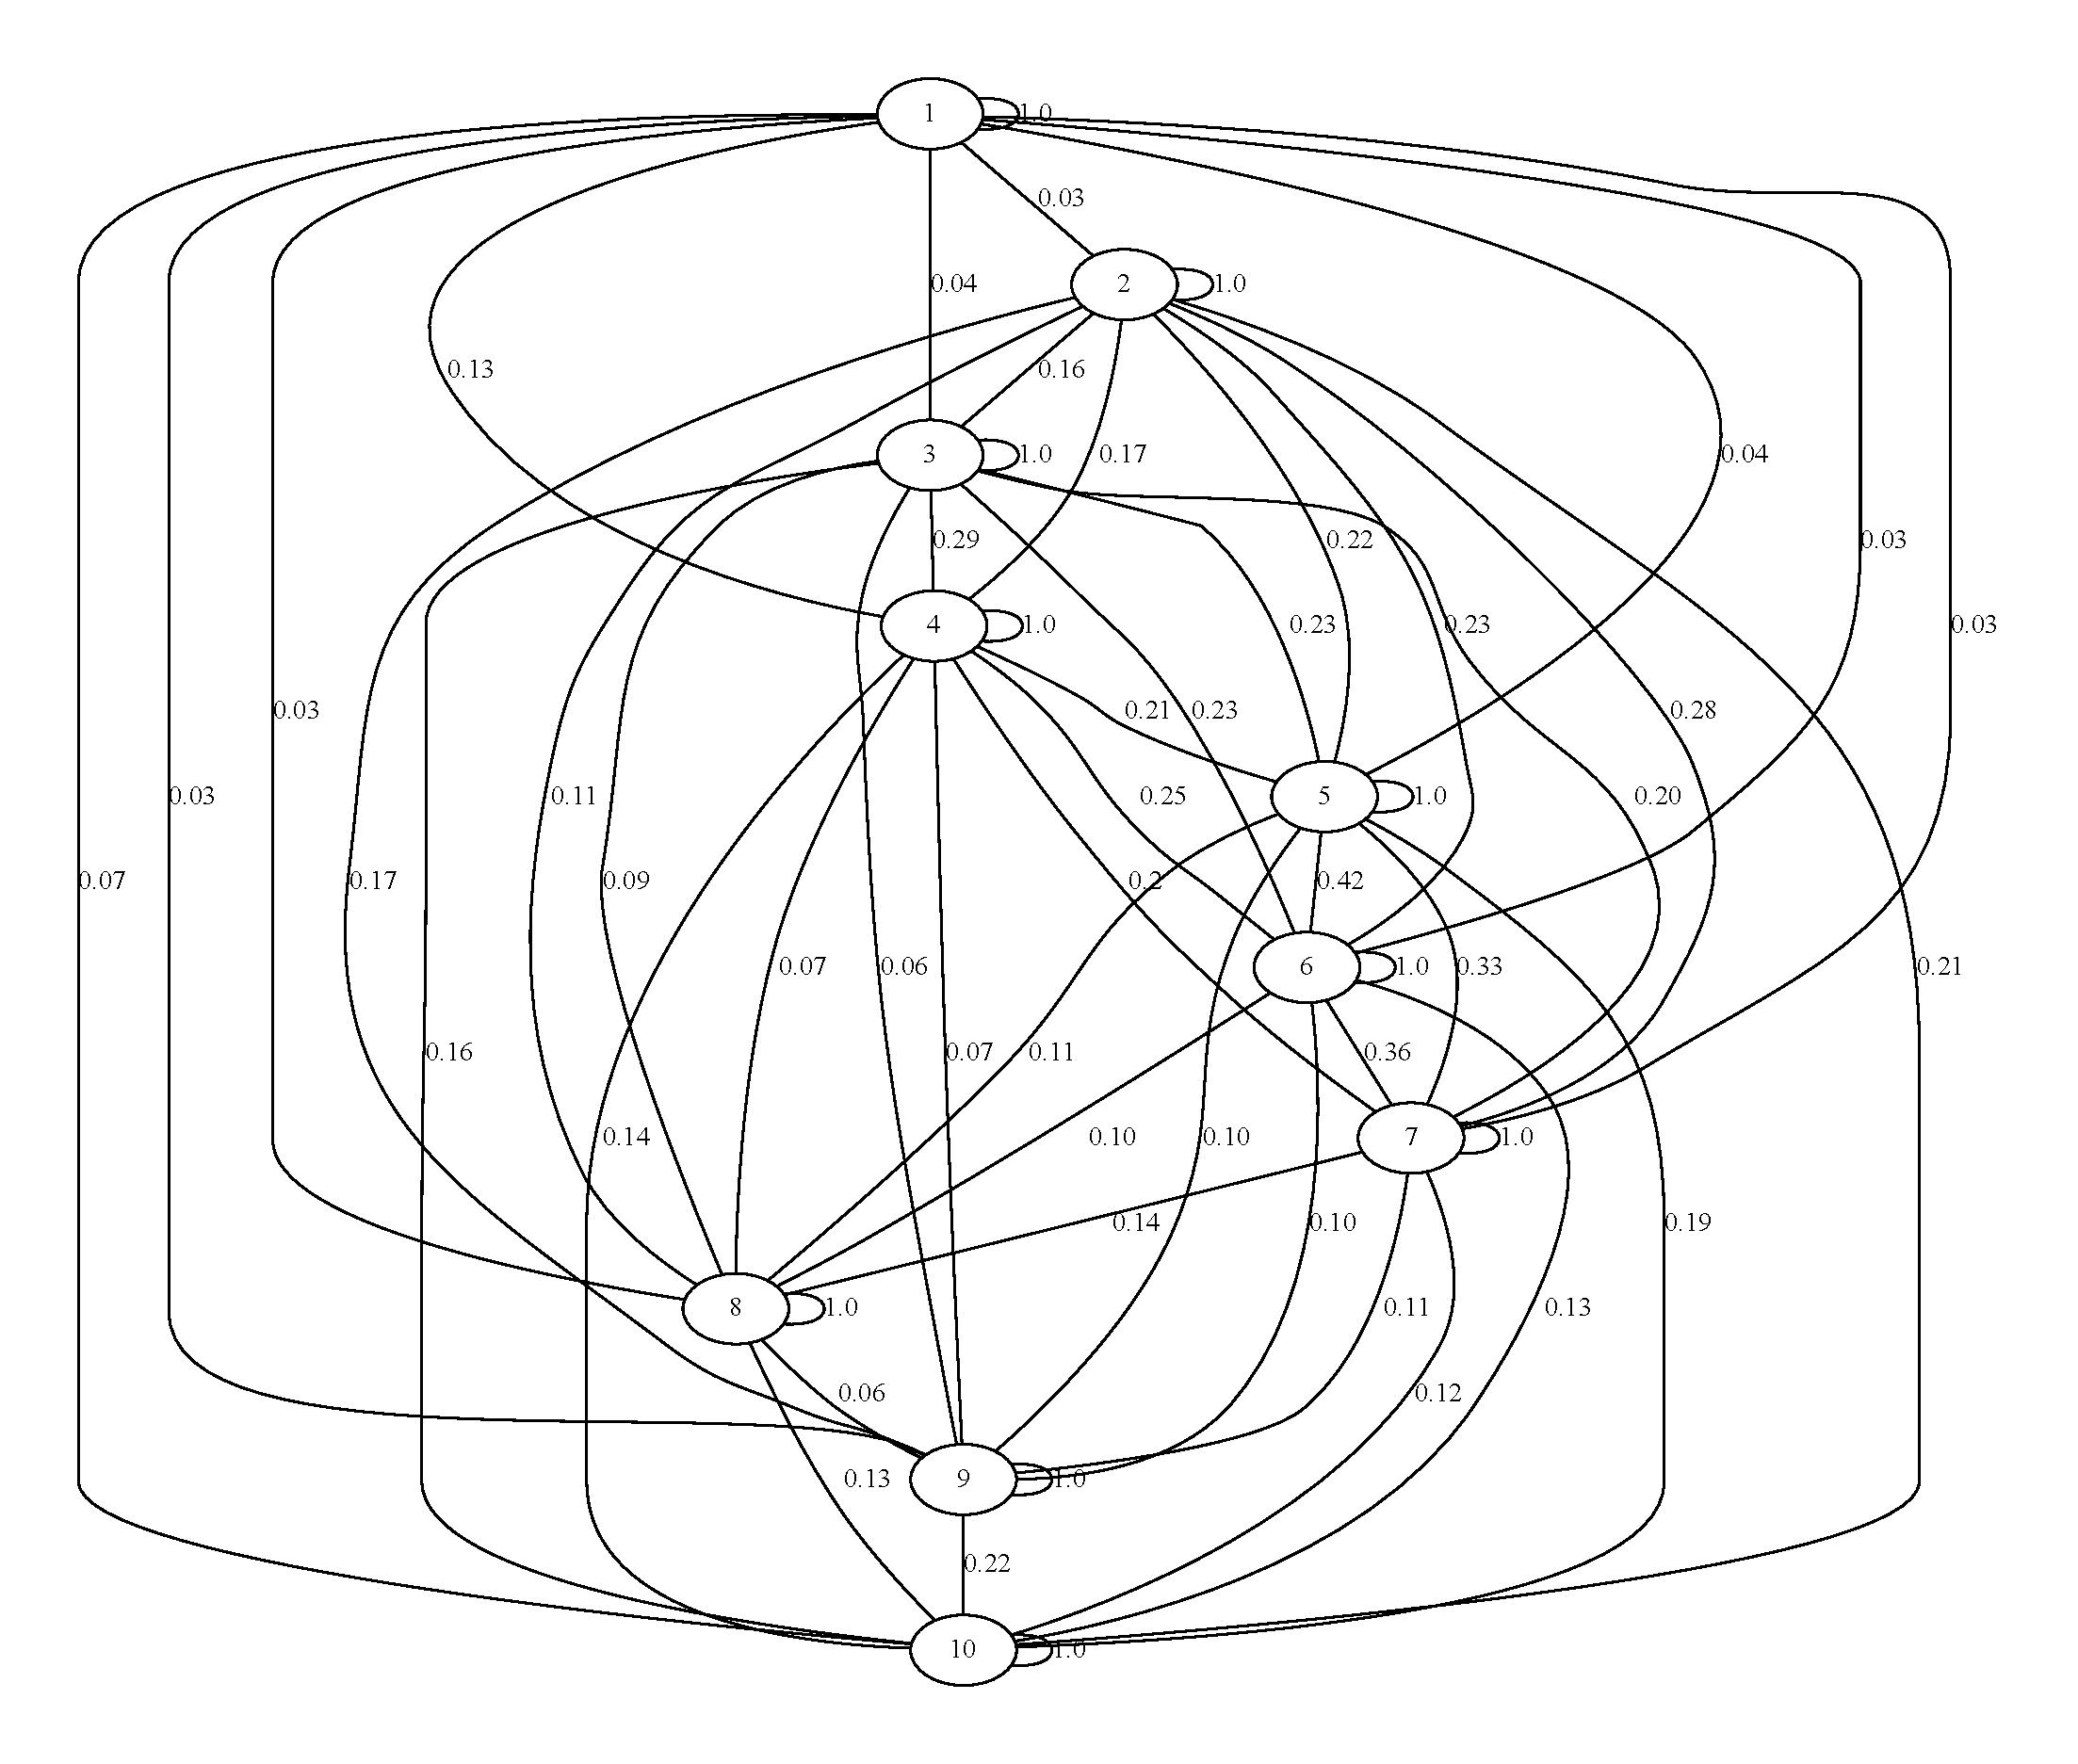
\includegraphics [width = \textwidth]{graphviz/au.pdf}
  \caption{A similarity graph representing pairwise similarities calculated by our tool between LMs shown in Table~\ref{table:ljms}.}
  \label{fig:au_graph}
\end{figure}




\section{Summary} \label{meth1-summary}
I have presented an approach for constructing a generalization from AUASTs of two LMs with special attention to logging calls via structural correspondence. This approach proceeds in three steps. First, several constraints have been applied on the selection of correspondences to prevent anti-unifying log method invocation nodes with any other types of nodes. Second, an approximation technique is employed to find the best correspondence for each AUAST node. Third, the anti-unification of two AUASTs is performed through the application of higher-order modulo theories over the AUAST structures. Furthermore, a measure of similarity has been developed that would provide us with useful information for the clustering phase.

An experimental study was conducted to evaluate the effectiveness of our anti-unification algorithm and the tool support in constructing an anti-unifier from AUASTs of each LJM pair in our test suite with a focus on logging calls and measuring similarity between them.



%This approach is implemented as an Eclipse plug-in which given two logged Java methods utilizes the Eclipse JDT framework to extract their ASTs. In order to be able to apply HOAUMT, we extended the AST structure to a higher-order structure, called AUAST, that would allow the insertion of variables in place of any nodes. We then applied the Jigsaw framework to identify potential correspondences between the two AUASTs and greedily determines the best correspondence for each node with the highest Jigsaw similarity.  Moreover




